
\documentclass[11pt,a4paper]{article}

\usepackage[utf8]{inputenc}
\usepackage[T1]{fontenc}
\usepackage{lmodern}
\usepackage[margin=2.5cm]{geometry}
\usepackage{setspace}
\usepackage{parskip}
\usepackage{graphicx}
\usepackage{float}
\usepackage{amsmath, amssymb}
\usepackage{booktabs}
\usepackage{array}
\usepackage{xcolor}
\usepackage{hyperref}
\usepackage{titlesec}
\usepackage{caption}
\usepackage{enumitem}
\usepackage{fancyhdr}
\usepackage{longtable}

\hypersetup{
    colorlinks=true,
    linkcolor=blue!50!black,
    urlcolor=blue!50!black,
    citecolor=blue!50!black
}

\setstretch{1.15}
\setlength{\parindent}{0pt}
\setlength{\parskip}{0.7em}

\definecolor{titleblue}{RGB}{27, 58, 99}
\definecolor{softgray}{RGB}{245, 245, 245}

\titleformat{\section}
  {\large\bfseries\color{titleblue}}
  {\thesection.}{0.6em}{}

\titleformat{\subsection}
  {\normalsize\bfseries\color{titleblue}}
  {\thesubsection.}{0.6em}{}

\pagestyle{fancy}
\fancyhf{}
\fancyhead[L]{Bioinformatics Article Summary}
\fancyhead[R]{Hierarchical marker genes selection in scRNA-seq analysis}
\fancyfoot[C]{\thepage}

\newcommand{\figureplaceholder}[2]{
\begin{figure}[H]
    \centering
    \fbox{\rule{0pt}{#1}\rule{0.9\linewidth}{0pt}}
    \caption{#2}
\end{figure}
}

\begin{document}

\begin{titlepage}
    \centering
    \vspace*{2cm}
    {\Huge\bfseries\color{titleblue} Article Summary \par}
    \vspace{0.4cm}
    {\LARGE Hierarchical marker genes selection in scRNA-seq analysis\par}
    \vspace{1cm}
    {\large Bioinformatics / scRNA-seq review\par}
    \vspace{1.5cm}

    \begin{minipage}{0.9\textwidth}
    \centering
    \setlength{\fboxsep}{12pt}
    \colorbox{softgray}{
        \parbox{0.85\textwidth}{
        \textbf{Article reference:} Sun, Y. \& Qiu, P. (2024). \textit{Hierarchical marker genes selection in scRNA-seq analysis}. \\
        \textbf{Main idea:} the authors propose a hierarchical marker gene selection strategy to overcome the limitations of the one-vs-all approach he one-vs-all approach, which is more classical, especially when cell types are closely related.
        }
    }
    \end{minipage}

    \vfill
    {\large Jef and Coline Clerbaux \par}
    \vspace{0.4cm}
    {\large April 2026 \par}
    \vfill
\end{titlepage}

\section{General context}

Single-cell RNA sequencing (scRNA-seq) is a technology that measures gene expression at the level of individual cells. Unlike older bulk RNA-seq methods, which average gene expression across large and heterogeneous populations of cells, scRNA-seq provides a much more precise view of cellular heterogeneity. This makes it especially useful for identifying new cell types, studying developmental trajectories, and investigating diseases such as cancer or immune disorders.

However, scRNA-seq generates very large and complex datasets. One central challenge is therefore to identify \textbf{marker genes}, namely genes whose expression helps distinguish one cell type from another. These marker genes are essential for annotating clusters obtained after unsupervised analysis and for giving them biological meaning.

\section{The problem addressed in the article}

A common strategy for identifying marker genes is the \textbf{one-vs-all} approach. In this framework, one cluster is compared against all the other clusters combined, and genes that are significantly more expressed in that cluster are selected as markers.

Although this strategy is widely used, it has a large limitation. When several clusters are \textbf{closely related cell types}, the selected marker genes will often overlap. In other words, they capture what these related clusters have in common rather than what truly distinguishes them. As a result, the one-vs-all strategy may fail to separate similar cell types accurately and may reduce the interpretability of the analysis.

To address this issue, the authors propose a \textbf{hierarchical marker gene selection method}. Instead of selecting markers for each cluster independently, they organize clusters into a hierarchy and identify marker genes at each split of this hierarchy. This allows them to define markers not only for individual cell types, but also for broader lineages and intermediate groups of related cell types.

\section{Introduction and main intuition}

The authors show that the classical Seurat one-vs-all heatmap often contains strong \textbf{off-diagonal signal}. In a marker heatmap, diagonal blocks represent marker genes strongly expressed in their intended cluster, which is desirable. By contrast, off-diagonal blocks indicate that these marker genes are also strongly expressed in other clusters, which suggests poor specificity.

The proposed hierarchical approach seeks to reduce this undesirable off-diagonal signal. The hierarchy starts from all cell types grouped together and progressively splits them into more specific branches. At each split, marker genes are redefined for the corresponding groups. The final result is an \textbf{assembled heatmap} in which marker gene expression is more structured and more specific to the appropriate clusters.

\begin{figure}[H]
    \centering
    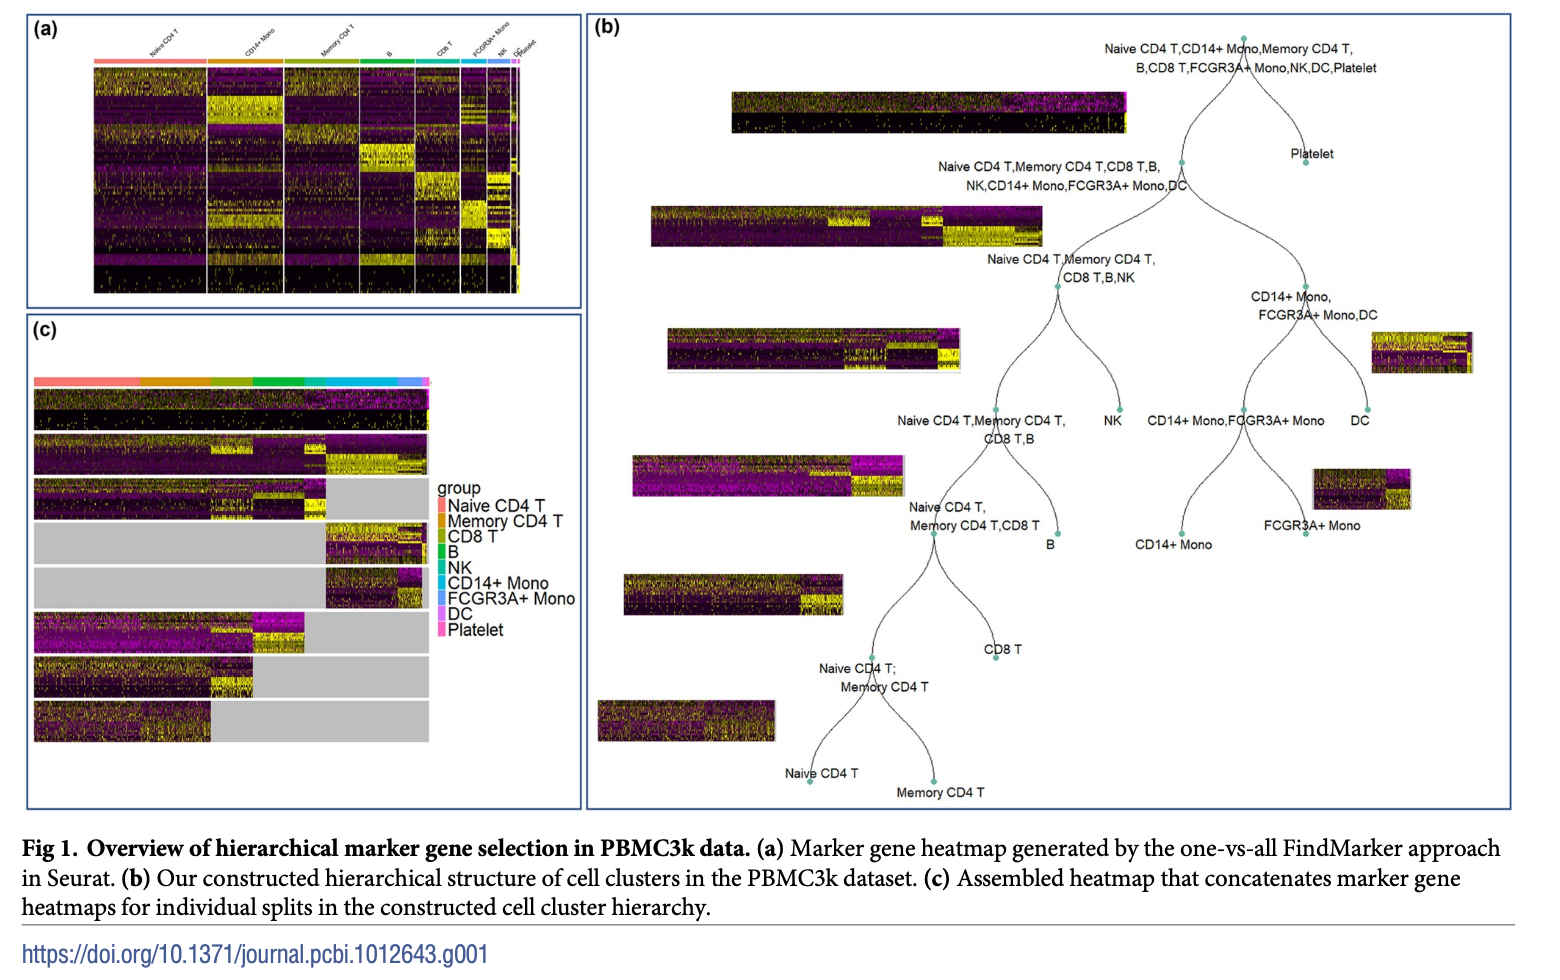
\includegraphics[width=\textwidth]{C1.png}
    \label{fig:figure1}
\end{figure}

\section{Project perspective}
In this project, we aim to further investigate the hierarchical marker gene selection method by comparing it with alternative approaches, and exploring how it behaves under different datasets and parameters.

\section{Methods}

\section{Results}

\section{Discussion}

\section{Conclusion}





\end{document}
